\begin{frame}
\frametitle{One mode of geometric variability}
\begin{columns}[c]
\column{0.5\textwidth}
Simulated images\par
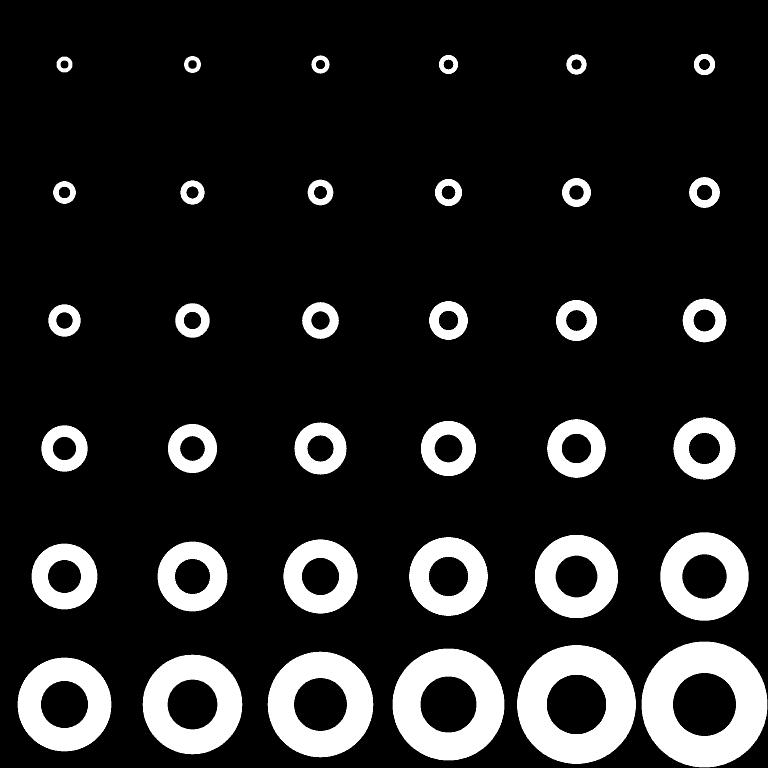
\includegraphics[height=0.9\textwidth]{circles}
\column{0.5\textwidth}
Principal components\par
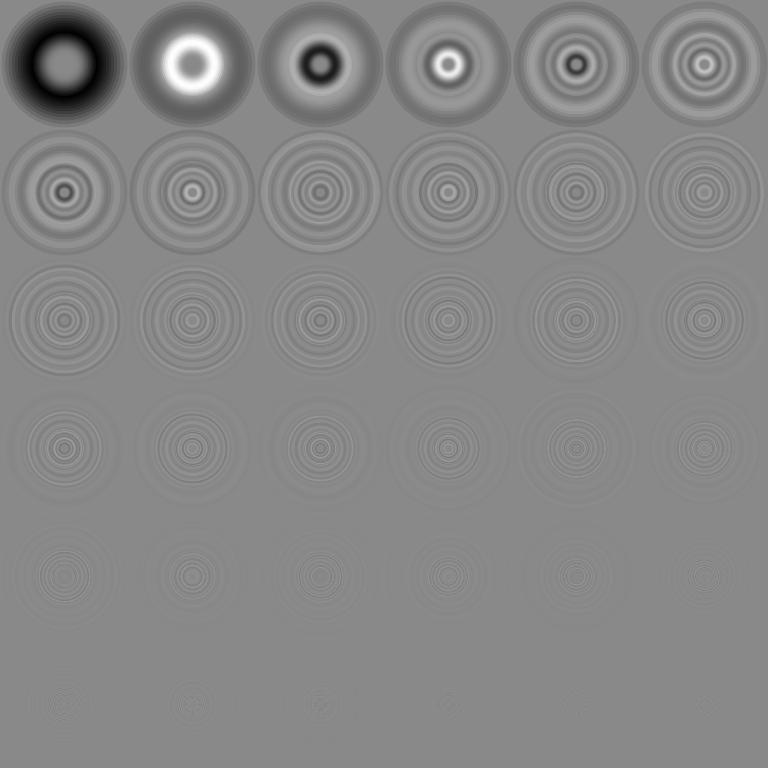
\includegraphics[height=0.9\textwidth]{circles_pca}
\end{columns}
A suitable model would reduce these data to a single dimension.
\end{frame}


\begin{frame}
\frametitle{Two modes of geometric variability}
\begin{columns}[c]
\column{0.5\textwidth}
Simulated images\par
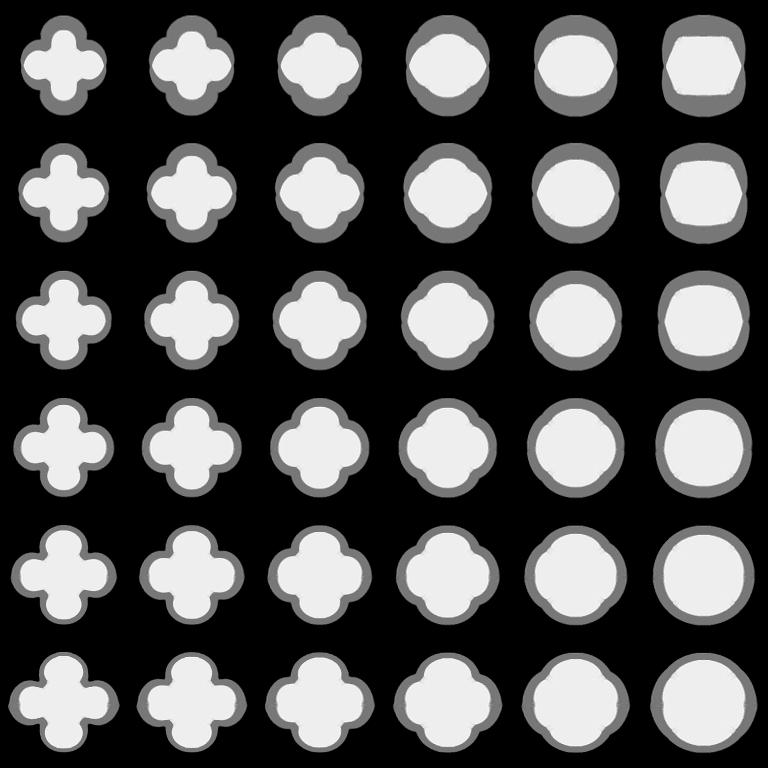
\includegraphics[height=0.9\textwidth]{things}
\column{0.5\textwidth}
Principal components\par
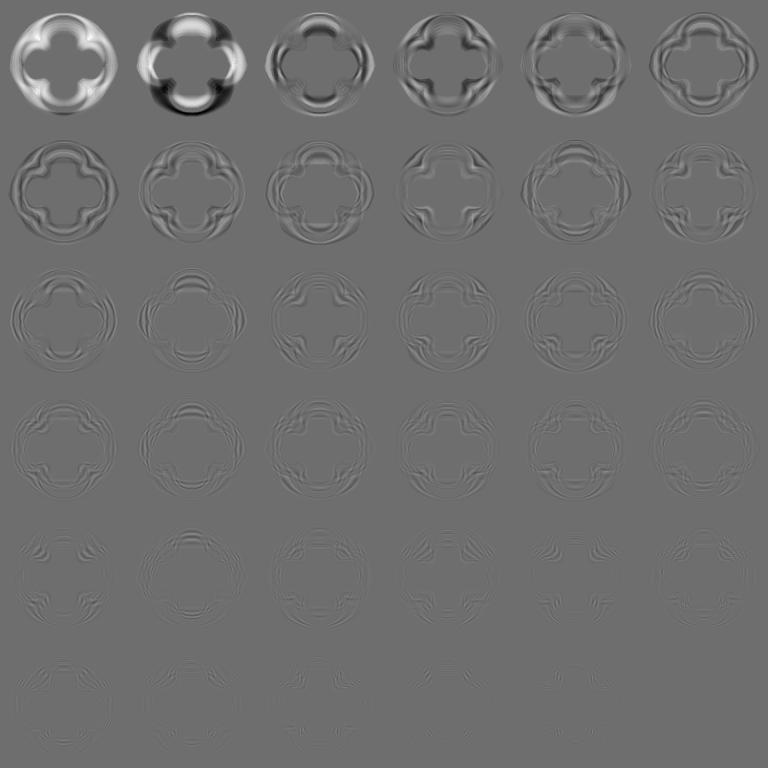
\includegraphics[height=0.9\textwidth]{things_pca}
\end{columns}
A suitable model would reduce these data to two dimensions.
\end{frame}

